\Chapter{Tervezés}
\Section{Modellek}

Modellek kapcsán első lépésben összegyűjtöttem számos OBJ file-t, egy részüknek az adatait \aref{fig:modellekt} táblázatban összegeztem.

\begin{table}[h]
\centering
\caption{Modellek táblázat}
\bigskip
\label{tab:modellek}
\begin{tabular}{|l|c|c|c|c|c|c|c|c|}
Modell neve& Csúcs & T.csúcs & N.csúcs & Lap & H.szög & N.szög \\
\hline
baby.obj & 12030 & 13154 & 12030 & 12028 & 0 & 12028 \\
barrel.obj & 9348 & 9674 & 5411 & 5887 & 0 & 5880	\\
bird.obj & 8758 & 9582 & 8685 & 8752 & 0 & 8752 \\
boat.obj & 102669 & 203174 & 66538 & 100624 & 1294 & 99330\\
butterfly.obj & 1394 &	8328 &	0 & 2776 &	2776 &	0 \\
camera.obj & 17000 & 18580 & 16788 & 16984 & 0 & 16984 \\
cat.obj & 35290 & 36525 & 35014 & 35288 & 0 &	35288 \\
chair.obj & 78906 & 111336 & 45764 & 83074 & 11352 & 71722 \\
coral.obj & 43212 & 51349 & 43211 & 43200 & 0 & 43200 \\
cube.obj & 8 & 4 & 6 & 12 & 12 & 0 \\
deer.obj & 39402 & 41696 & 38642 & 39384 & 0 & 39384 \\
dog.obj & 35986 & 37096 & 35983 & 35984 & 0 & 35984 \\
dolphin.obj & 7338 & 7815 & 7337 & 7336 & 0 & 7336 \\
door.obj & 2058 & 2456 & 629 & 2152 &	220 & 1932 \\
lion.obj & 64558 & 67131 & 64556 & 64536 & 0 & 64536 \\
monkey.obj & 47490 & 49505 & 47490 & 47488 & 0 & 47488 \\
necklace.obj & 85592 &	94527 & 83931 & 85592 & 0 & 85592 \\
penguin.obj & 7494 & 7961 & 7493 & 7488 & 0 & 7488 \\
skull.obj & 40062 & 42682 & 40062 & 40728 & 1440 & 39288 \\
wrench.obj & 11568 & 13326 & 10508 & 11568 & 0 & 11568 \\
\hline
\end{tabular}
\label{fig:modellekt}
\end{table}

\Aref{fig:modellekt} tábázat modelljeit a \url{https://free3d.com/} oldalról szereztem be, ahol rengetek modell megtalálható. Ezeken a modelleken fellépő hibákat illetve különböző modellek kompatibilitási problémáit vizsgáltam.

Vizsgálat során az első szembetűnő dolog az volt, hogy ezek az objektumok komplexitásukban, jelentősen eltérnek egymástól. Voltak köztük olyan objektumok, amik viszonylag kevés komponensből állnak össze és voltak olyanok is, amik ezekhez képest jelentősen több elemből.
Természetesen az oldalon található modell fájlok többsége teljesen jól működik, de akadtak köztük hibásak is.

Rendszereztem őket az alábbi kategóriákba:
\begin{itemize}
\item \textit{Helyes modellek}:
A megjelenítés tökéletesen megtörtént.
\item \textit{Javítható hibát tartalmazó modellek}:
A modellnek olyan javítható hibája van, ami a program segítségével majd javításra kerülhet.
\item \textit{Nem javítható hibák tartalmazó modellek}:
A modellnek olyan hibája van, ami nem kerülhet javításra a program segítségével.
\end{itemize}
\bigskip

\Section{Saját modell struktúra megtervezése}

Ennél a lépésnél megvizsgáltam, és figyelembe vettem az általam vizsgált modell betöltők struktúrális felépítését, és a következő konzekvenciát szűrtem le.
Az általam megvizsgált modell betöltők tárolási módjai elég hasonlóak. Az objektum adatait egy közös modell struktúrában tárolják, ezt feltöltő adatokat pedig alstruktúrákban.

A saját tervezésű program az OBJ fájl adatait egy közös model struktúrában tárolja. A struktúrák és alstruktúrák felépítése és viszonyai \aref{fig:struct}. ábrán láthatók.

\begin{figure}[h]
\centering
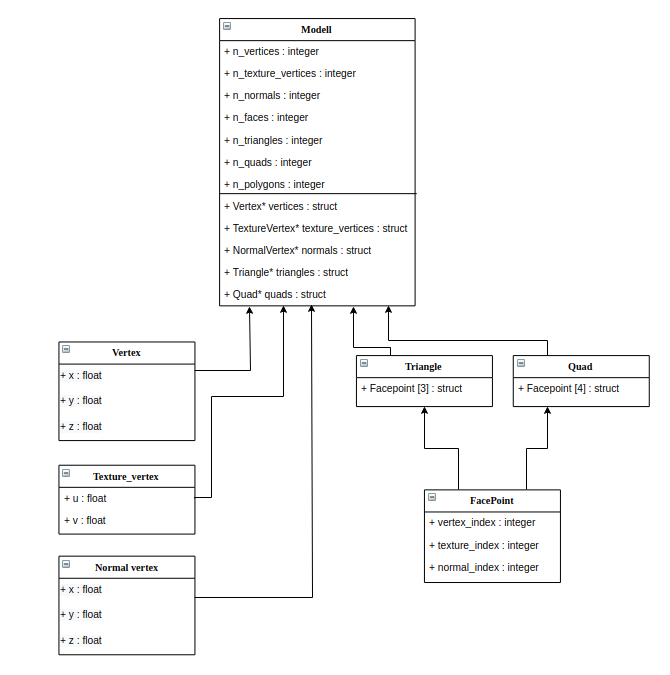
\includegraphics[width=\textwidth]{images/struct.png}
\caption{A saját adatstruktúra felépítése a modellek adatainak tárolásához}
\label{fig:struct}
\end{figure}

Az integer típusú \texttt{n\_vertices}, \texttt{n\_texture\_vertices}, \texttt{n\_normals}, \texttt{n\_faces} illetve \texttt{n\_triangles}, \texttt{n\_quads} és \texttt{n\_polygons} változók feltöltésre kerülnek az OBJ fájl különböző változótípus darabasznámainak összeszámlálásával.
\begin{python}
typedef struct Model
{
    int n_vertices;
    int n_texture_vertices;
    int n_normals;
    int n_faces;
    int n_triangles;
    int n_quads;
    int n_polygons;
} Model;
\end{python}
Ezt követően a \texttt{n\_vertices} számával közvetlen kiolvasásra kerülnek a \texttt{Vertex} struktúra különböző csúcspontjai.
\begin{python} 
typedef struct Vertex
{
    double x;
    double y;
    double z;
} Vertex;
\end{python}
Hasonlóan a \texttt{Vertex} struktúrához a \texttt{TextureVertex} csúcspontjai is kiolvasásra kerülnek az \texttt{n\_texture\_vertices} darabszámával.
\begin{python}
typedef struct TextureVertex
{
    double u;
    double v;
} TextureVertex;
\end{python}
Majd az előzőekhez hasonlóan a \texttt{NormalVertex}  struktúra csúcspontjai is feltöltődnek az \texttt{n\_normals} darabszámmal.
\begin{python}
typedef struct NormalVertex
{
    double x;
    double y;
    double z;
} NormalVertex;
\end{python}
Végül a \texttt{Triangle} és \texttt{Quad} struktúrák is feltöltésre kerülnek, \texttt{FacePoint} struktúra segítségével \texttt{n\_triangles} , illetve \texttt{n\_quads} darabszámmal.
\begin{python}
typedef struct FacePoint
{
    int vertex_index;
    int texture_index;
    int normal_index;
} FacePoint;

typedef struct Triangle
{
    struct FacePoint points[3];
} Triangle;

typedef struct Quad
{
    struct FacePoint points[4];
} Quad;
\end{python}
Az összes adat így a \texttt{Model} struktúrában kerül eltárolásra. Ennek előnye, hogy egy közös helyet kap az OBJ fájl összes fontos adata, így egyszerűbben lehet rájuk hivatkozni, illetve a modellen történő szükséges változásokat így könnyebben elvégezhetjük.
\begin{python}
typedef struct Model
{
    int n_vertices;
    int n_texture_vertices;
    int n_normals;
    int n_faces;
    int n_triangles;
    int n_quads;
    int n_polygons;
    struct Vertex* vertices;
    struct TextureVertex* texture_vertices;
    struct NormalVertex* normals;
    struct Triangle* triangles;
    struct Quad* quads;
}Model;
\end{python}

\Section{Elem indexelés}

\Aref{fig:index_}. ábrán látható az egyes lap elemek különböző csúcsok koordinátjának összeolvasására szolgáló funkció megtervezése.

\begin{figure}[h]
\centering
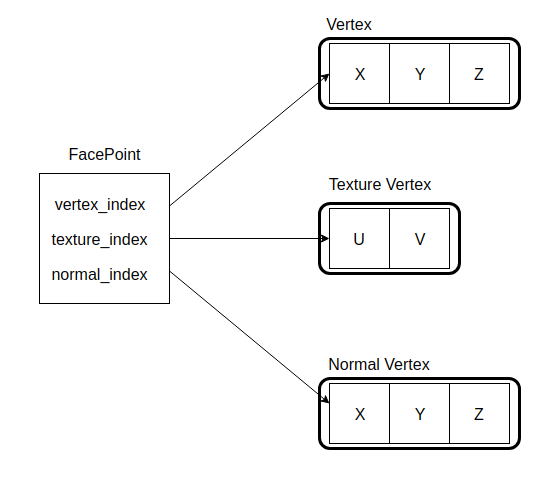
\includegraphics[scale=0.5]{images/point.png}
\caption{Elem indexelés.}
\label{fig:index_}
\end{figure}

\noindent Ennek a segítségével fogja a program összeállítani a különböző síkidomokat megjelenítés során.

A \texttt{Triangle} és \texttt{Quad} struktúrák indexhelyesen mutatnak az egyes csúcsok koordinátáira.
Például, az első fejezetben bemutatott négyszög objektum esetében:
\begin{python} 
v 0.0 0.0 0.0
v 1.0 0.0 0.0
v 1.0 1.0 0.0
v 0.0 1.0 0.0

vt 0.0 0.0
vt 1.0 0.0
vt 1.0 1.0
vt 0.0 1.0

vn 1.0 0.0 0.0 

f 1/1/1 2/2/1 3/3/1 4/4/1
\end{python}
A lap (\textbf{f}) eleme először mutat a \textbf{v}, \textbf{vt}, \textbf{vn} (\texttt{1, 1, 1}) koordinátáira, ami ennél a példánál (\texttt{v 0.0 0.0 0.0, vt 0.0 0.0, vn 1.0 0.0 0.0}).
A második esetnél \textbf{v}, \textbf{vt}, \textbf{vn} (\texttt{2, 2, 1}) koordinátáira (\texttt{v 1.0 0.0 0.0, vt 1.0 0.0, vn 1.0 0.0 0.0}), így végighaladva az összes lap elemen.
